\newpage
\section{Suddivisione del lavoro}
I componenti del gruppo dovranno rivestire ciascuno, almeno una volta, tutti i ruoli specificati nell'\textit{organigramma\ped{G}}.
Durante le varie fasi ogni componente può ricoprire più ruoli, anche contemporaneamente, purchè non si presentino dei conflitti di interesse tra le attività svolte. Ad esempio un componente non potrà essere \textit{\Ver} del codice scritto da egli stesso.
\paragraph{Legenda}
\begin{itemize}
\item\textbf{PM:} \Pm
\item\textbf{AM:} \Am
\item\textbf{AN:} \An
\item\textbf{PT:} \Prog
\item\textbf{PR:} \Progr
\item\textbf{VE:} \Ver
\end{itemize}
\subsection{\ARM}

Nell'attività di \ARM\ ciascun componente dovrà rivestire i seguenti ruoli:


\begin{table}[h]
	\begin{center}
		\begin{tabular}{|c|c|c|c|c|c|c|c|}
			\hline
			\textbf{Nominativo} & \multicolumn{6}{c|}{\textbf{Ore per ruolo}} & \textbf{Ore totali} \\
					& PM & AM & AN & PT & PR & VE & \\
			\hline
			\FB		&	 &	4 &	10 &  	&	 & 12 &	26	\\
			\hline
			\RM		& 5 &	  &	6  & 	&	 & 15 &	26	\\
			\hline
			\SL		& 8  & 6  &	11 &	 &	 &	  &	25	\\
			\hline
			\DC		&	 & 1  &	8  &	&	 & 17 &	26	\\
			\hline
			\LD 	& 7	 & 2  &	9 &	&	 & 7  &	25	\\
			\hline
			\MT		& 	 &    &	12 &	 &	 & 14 &	26	\\
			\hline
			\ND 	&	 & 6  &	19 & &	 &	  & 25	\\
			\hline
		\end{tabular}
	\end{center}
	\caption{Costo per ruolo, \ARM}
\end{table}

\begin{figure}[H]
	\centering 
	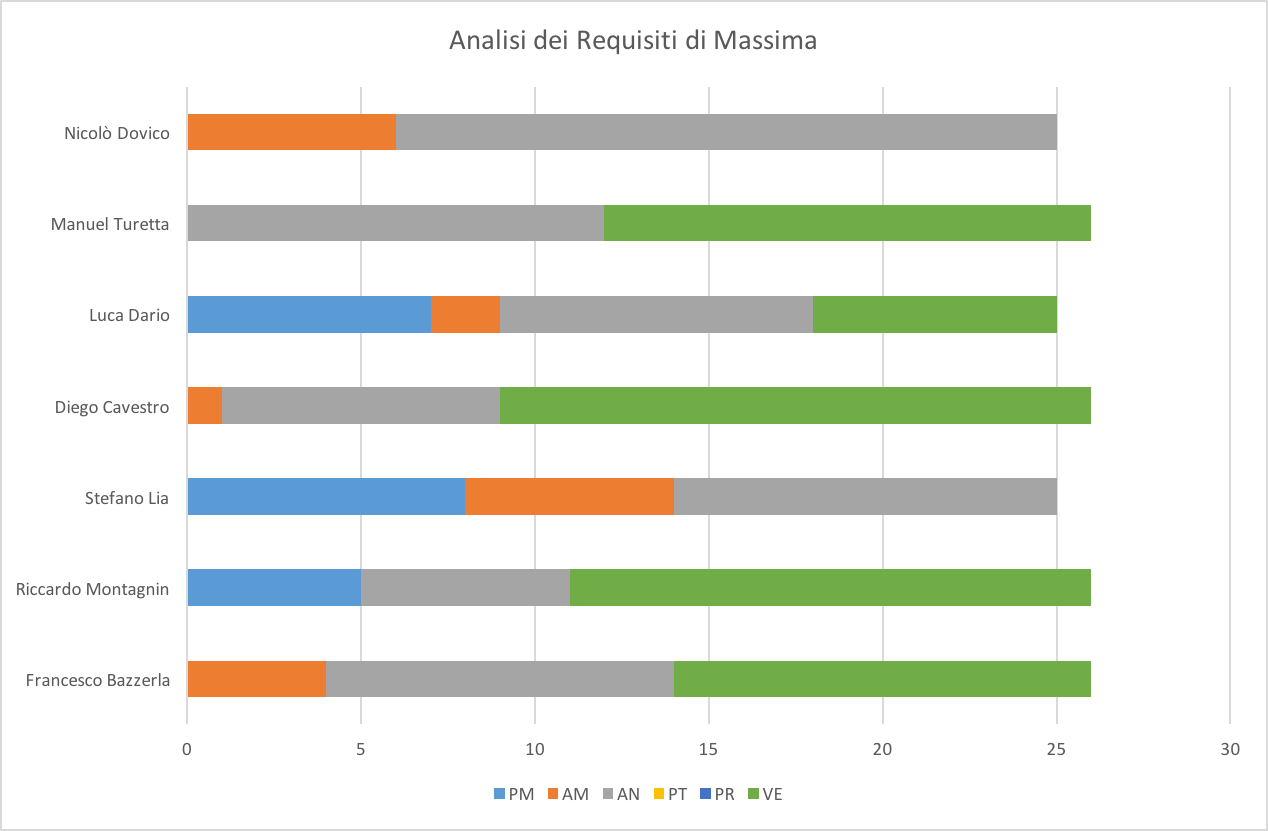
\includegraphics[scale=0.55]{Immagini/GraficiPianoLavoro/ARM.png}
	\caption{Incidenza ore per membro, \ARM}
\end{figure}

\newpage
\subsection{\ARD}
Nell'attività di \ARD ciascun componente dovrà rivestire i seguenti ruoli:

\begin{table}[h]
	\begin{center}
		\begin{tabular}{|c|c|c|c|c|c|c|c|}
			\hline
			\textbf{Nominativo} & \multicolumn{6}{c|}{\textbf{Ore per ruolo}} & \textbf{Ore totali} \\
					& PM & AM & AN & PT & PR & VE & \\
			\hline
			\FB		& 	 &	  &	6  &	&	 & 1  &	7 \\
			\hline
			\RM		&	 & 1  &	6  &	&	 &	  &	7	\\
			\hline
			\SL		& 2	 &	  &	   &	&	 & 6  &	8	\\
			\hline
			\DC		&	 &	  &	7  &	&	 & 	  &	7	\\
			\hline
			\LD 	&	 &	  &	6  &	&	 & 1  &	7	\\
			\hline
			\MT		& 	 & 2  &	5  &	&	 &	  &	7	\\
			\hline
			\ND 	& 1	 &	  &	   &	&	 & 6  &	7	\\
			\hline
		\end{tabular}
	\end{center}
	\caption{Costo per ruolo, \ARD}
\end{table}

\begin{figure}[H]
	\centering 
	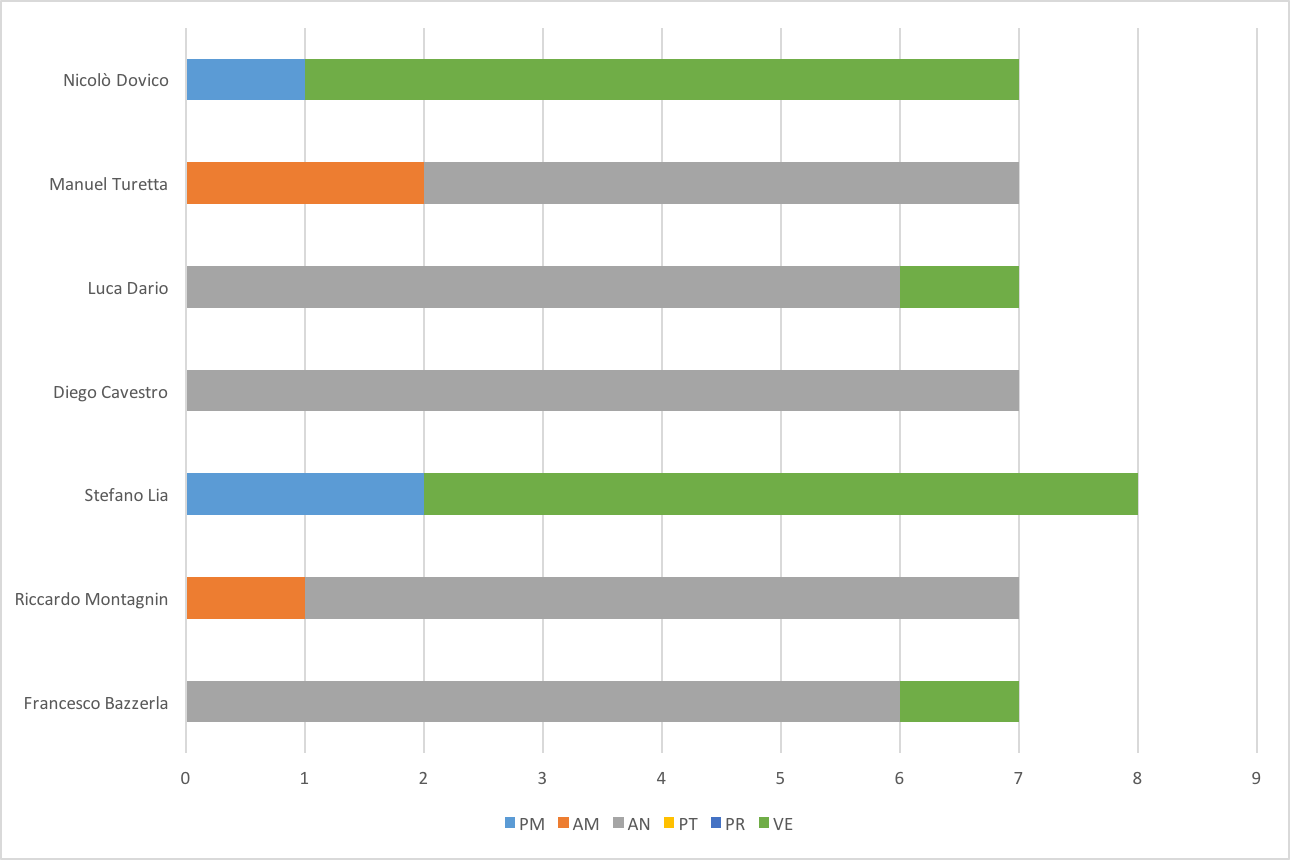
\includegraphics[scale=0.7]{Immagini/GraficiPianoLavoro/ARD.png}
	\caption{Incidenza ore per membro, \ARD}
\end{figure}

\newpage
\subsection{\PA}
Nel periodo di \PA\ ciascun componente del gruppo dovrà rivestire i seguenti ruoli:

\begin{table}[h]
	\begin{center}
		\begin{tabular}{|c|c|c|c|c|c|c|c|}
			\hline
			\textbf{Nominativo} & \multicolumn{6}{c|}{\textbf{Ore per ruolo}} & \textbf{Ore totali} \\
					& PM & AM & AN & PT & PR & VE & \\
			\hline
			\FB		&	 &	  &	   & 20	&	 & 8  &	28	\\
			\hline
			\RM		&	 & 2  &	   & 18	&  	 & 8 & 28	\\
			\hline
			\SL		&	 &	  &	   & 15	&	 & 13 &	28	\\
			\hline
			\DC		&	 & 5  &	   & 23	&	 & 	  &	28	\\
			\hline
			\LD 	& 3	 &	  &	   & 11	&	 & 15 &	29	\\
			\hline
			\MT		& 3	 &	  &	   & 13	&	 & 12 &	28	\\
			\hline
			\ND 	&	 &	  &	   & 20	&	 & 9  & 29	\\
			\hline
		\end{tabular}
	\end{center}
	\caption{Costo per ruolo, \PA}
\end{table}

\begin{figure}[H]
	\centering 
	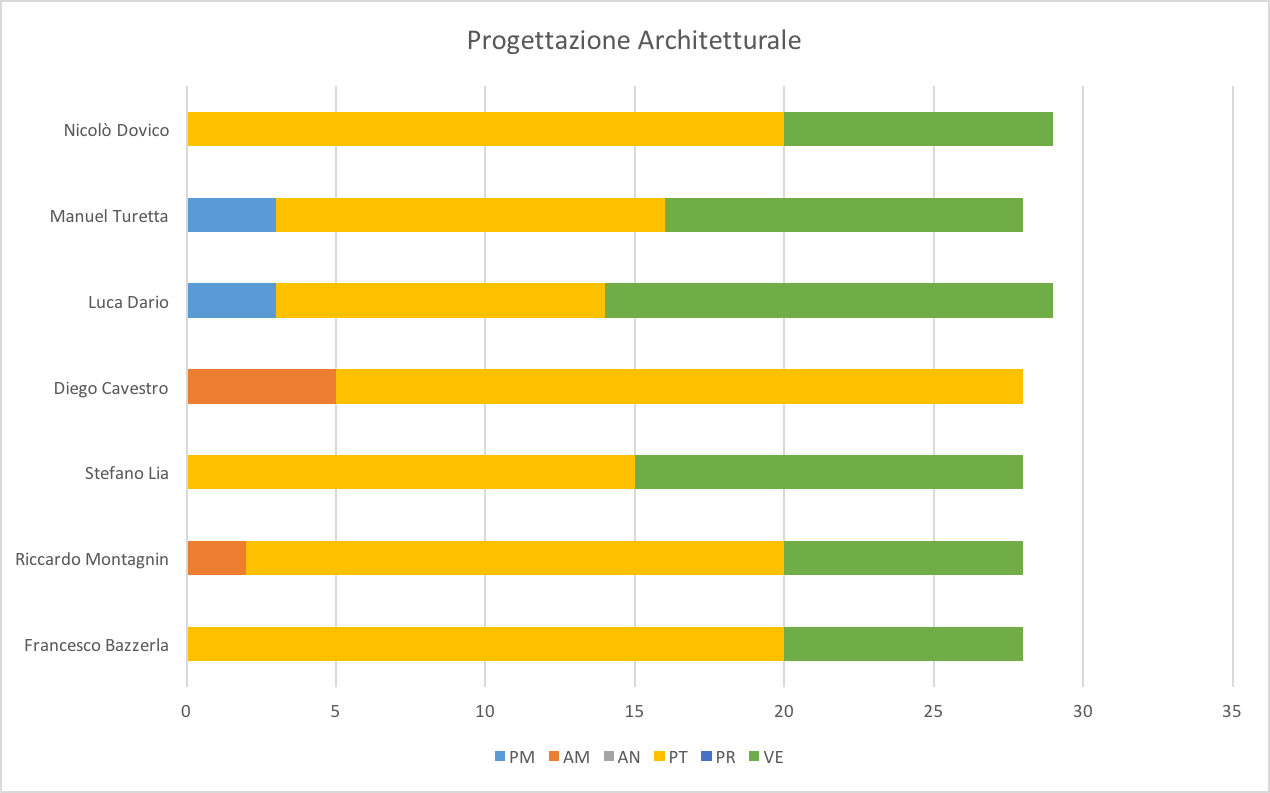
\includegraphics[scale=0.7]{Immagini/GraficiPianoLavoro/PA.png}
	\caption{Incidenza ore per membro, \PA}
\end{figure}

\newpage
\subsection{\PD}
Nel periodo di \PD\ ciascun componente del gruppo dovrà rivestire i seguenti ruoli:

\begin{table}[h]
	\begin{center}
		\begin{tabular}{|c|c|c|c|c|c|c|c|}
			\hline
			\textbf{Nominativo} & \multicolumn{6}{c|}{\textbf{Ore per ruolo}} & \textbf{Ore totali} \\
					& PM & AM & AN & PT & PR & VE & \\
			\hline
			\FB		& 4  &	  &	   & 5	&	 & 8  &	17	\\
			\hline
			\RM		&	 &	  &	   & 9	&	 & 8 & 17	\\
			\hline
			\SL		&	 & 5  &	   & 5	&	 & 8  &	18	\\
			\hline
			\DC		& 3	 &	  &	   & 14	&	 & 	  &	17	\\
			\hline
			\LD 	&	 &	  &	   & 7	&	 & 10  &	17	\\
			\hline
			\MT		& 	 & 	  &	   & 10	&	 & 8  &	18	\\
			\hline
			\ND 	&	 & 2  &	   & 15	&	 &	  & 17	\\
			\hline
		\end{tabular}
	\end{center}
	\caption{Costo per ruolo, \PD}
\end{table}

\begin{figure}[H]
	\centering 
	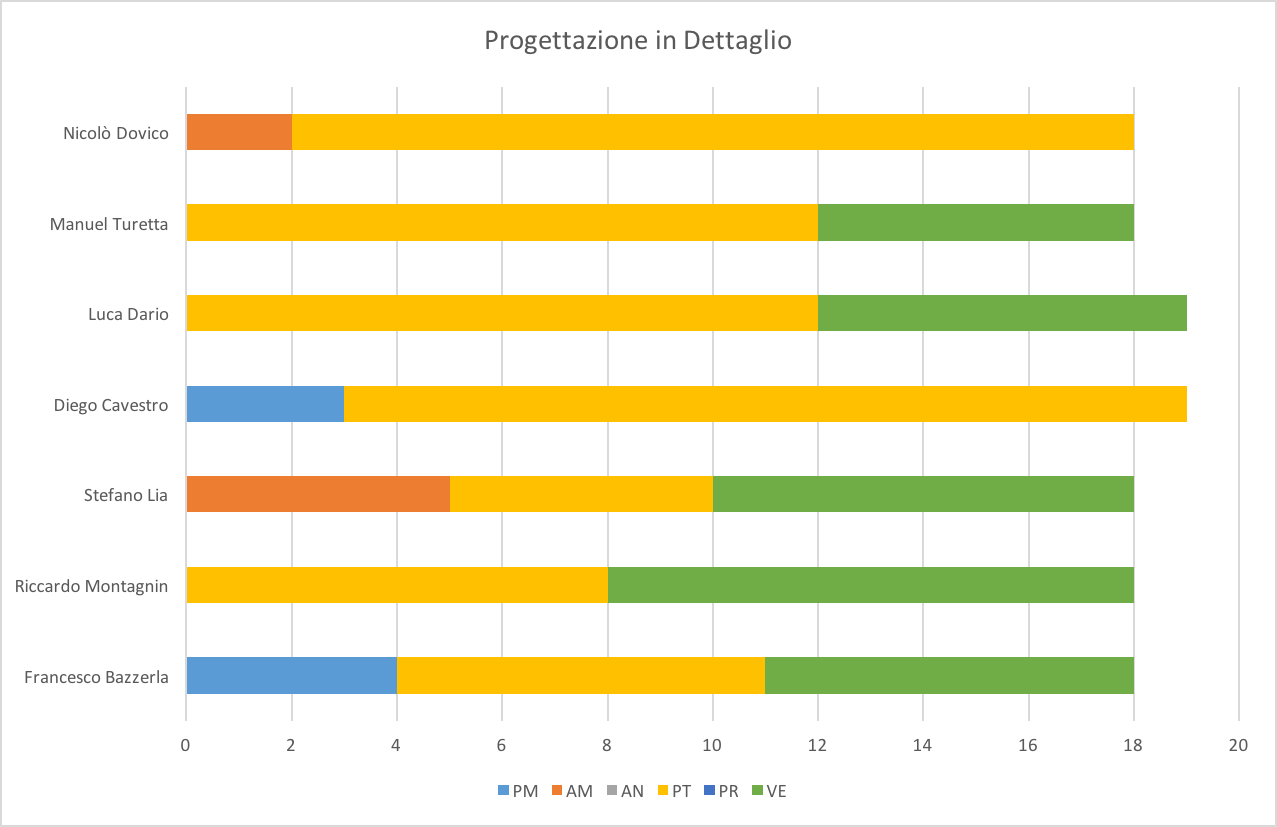
\includegraphics[scale=0.7]{Immagini/GraficiPianoLavoro/PD.png}
	\caption{Incidenza ore per membro, \PD}
\end{figure}

\newpage
\subsection{\COD}
Nel periodo di \COD\ ciascun componente del gruppo dovrà rivestire i seguenti ruoli:

\begin{table}[h]
	\begin{center}
		\begin{tabular}{|c|c|c|c|c|c|c|c|}
			\hline
			\textbf{Nominativo} & \multicolumn{6}{c|}{\textbf{Ore per ruolo}} & \textbf{Ore totali} \\
					& PM & AM & AN & PT & PR & VE & \\
			\hline
			\FB		&	 &	  &	   & 10	& 22 &	6  &	38	\\
			\hline
			\RM		&	 &	  &	   & 	& 16 & 20 & 36	\\
			\hline
			\SL		& 2  &	  &	   & 11	& 19 & 3  &	35	\\
			\hline
			\DC		&	 &	  &	   &	& 14	 & 22 &	36	\\
			\hline
			\LD 	&	 &	  &	   &	& 23 & 13 &	36	\\
			\hline
			\MT		& 	 & 2  &	   &	& 23 & 10  &	35	\\
			\hline
			\ND 	& 9	 & 4  &	   &	& 20 & 3   & 36	\\
			\hline
		\end{tabular}
	\end{center}
	\caption{Costo per ruolo, \COD}
\end{table}

\begin{figure}[H]
	\centering 
	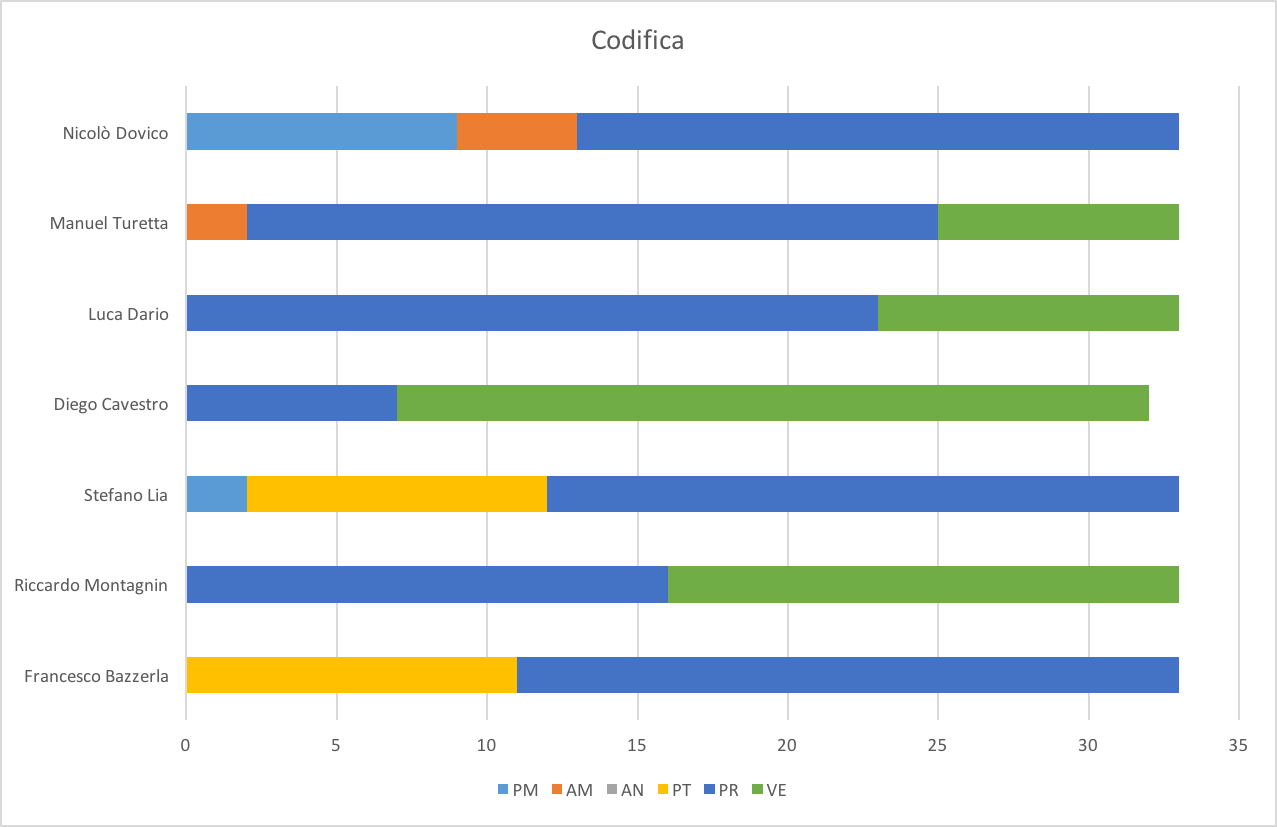
\includegraphics[scale=0.7]{Immagini/GraficiPianoLavoro/COD.png}
	\caption{Incidenza ore per membro, \COD}
\end{figure}

\newpage
\subsection{\VV}
Nel periodo di \VV{} ciascun componente del gruppo dovrà rivestire i seguenti ruoli:

\begin{table}[h]
	\begin{center}
		\begin{tabular}{|c|c|c|c|c|c|c|c|}
			\hline
			\textbf{Nominativo} & \multicolumn{6}{c|}{\textbf{Ore per ruolo}} & \textbf{Ore totali} \\
					& PM & AM & AN & PT & PR & VE & \\
			\hline
			\FB		& 5  &	  &	   &	&	 & 10 &	15	\\
			\hline
			\RM		& 7	 &	  &	   &	&	 & 10 & 17	\\
			\hline
			\SL		&	 & 6  &	   &	&	 & 10 &	16	\\
			\hline
			\DC		& 1	 &	  &  & 3  &	3 & 10 &	17	\\
			\hline
			\LD 	&	 &	  &	   & 3	&	3 & 10 &	16	\\
			\hline
			\MT		& 1 	 &	  &	   & 3	&	3 & 10 &	17	\\
			\hline
			\ND 	&	 & 2  &	   & 3	&	2 & 9 & 16	\\
			\hline
		\end{tabular}
	\end{center}
	\caption{Costo per ruolo, \VV}
\end{table}

\begin{figure}[H]
	\centering 
	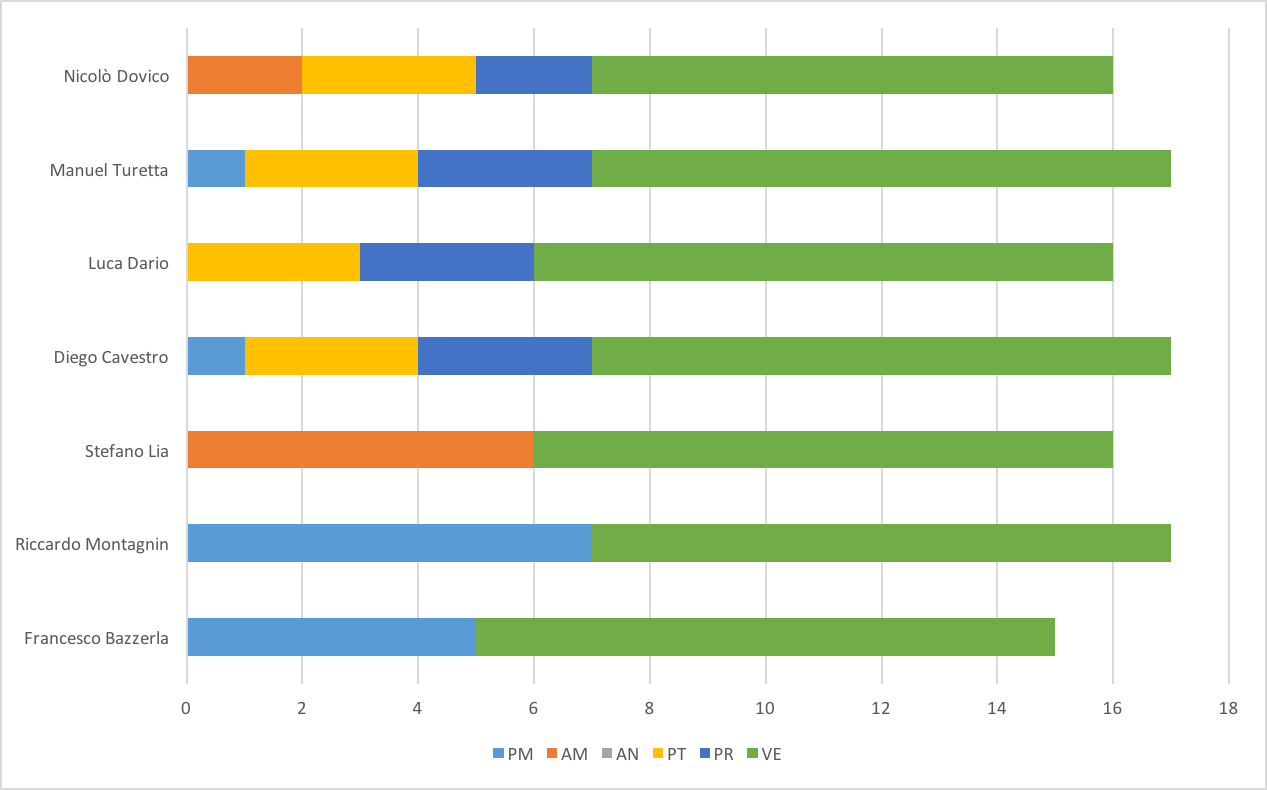
\includegraphics[scale=0.7]{Immagini/GraficiPianoLavoro/VV.png}
	\caption{Incidenza ore per membro, \VV}
\end{figure}

\newpage
\subsection{Totali}
La tabella seguente illustra le ore totali che ogni componente dedicherà per il progetto, mettendo in evidenza anche quelle che verranno poi rendicontate. Le ore non rendicontate corrispondono alle ore dedicate al primo periodo (\ARM) che, come già esplicato in precedenza, rappresenta l'investimento iniziale del \termine{gruppo} per aggiudicarsi il capitolato e comprendono, oltre ad attività di auto-apprendimento, tutte le attività svolte nel periodo di \ARM\ (§3.2.1).
\begin{table}[h]
	\begin{center}
		\begin{tabular}{|c|c|c|c|c|c|c|c|c|}
			\hline
			\multirow{2}{*} {\textbf{Nominativo}} & & \multicolumn{6}{c|}{\textbf{Ore per ruolo}} & \multirow{2}{*}{\textbf{Ore totali}} \\
			& & PM & AM & AN & PT & PR & VE & \\
			\hline
			\multirow{2}{*}{\FB}		&	Rendicontate	&	9	&	0	&	6	&	35 & 22	&	33 & 105	\\
			\cline{2-9}
			&	Totali			&	9	& 4	&	16	&	35	&	22	& 45 &	131	\\
			\hline
			\multirow{2}{*}{\RM}	&	Rendicontate	&	7 &	3	&	6	&	27	&	16	&  46	&	105	\\
			\cline{2-9}
			&	Totali			&	12	&	3	&	12	&	27	&	16	& 	61	&	131	\\
			\hline
			\multirow{2}{*}{\SL}	&	Rendicontate	&	4	&	11	&	0	&	31	&	19	&	40	&	105	\\	
			\cline{2-9}
			&	Totali			&	12	&	17	&	11	&	31	&	19	&	40	&	130	\\
			\hline
			\multirow{2}{*}{\DC}	&	Rendicontate	&	4	&	5	&	7	&	40	&	17	&	32	&	105	\\	
			\cline{2-9}
			&	Totali			&	4	&	6	&	15	&	40	&	17	&	49	&	131	\\
			\hline
			\multirow{2}{*}{\LD}		&	Rendicontate	&	3	&	0	&	6	& 21	&	26	& 	49	&	105	\\	
			\cline{2-9}
			&	Totali			&	10	&	2	&	15	&	21	&	26	& 	56	&	130	\\
			\hline
			\multirow{2}{*}{\MT}	&	Rendicontate	&	4	&	4	&	5	&	26	&	26	& 	40	&	105	\\
			\cline{2-9}
			&	Totali			&	4	&	4	&	17	&	26	&	26	& 	54	&	131	\\
			\hline
			\multirow{2}{*}{\ND}	&	Rendicontate	&	10	&	8	&	0	&	38	&	22	& 	27	&	105	\\	
			\cline{2-9}
			&	Totali	&	10	&	14	&	19	&	38	&	22	& 	27	&	130	\\
			\hline
		\end{tabular}
	\end{center}
	\caption{Ore per componente per ruolo, rendicontate e totali}
\end{table}

\begin{figure}[H]
	\centering 
	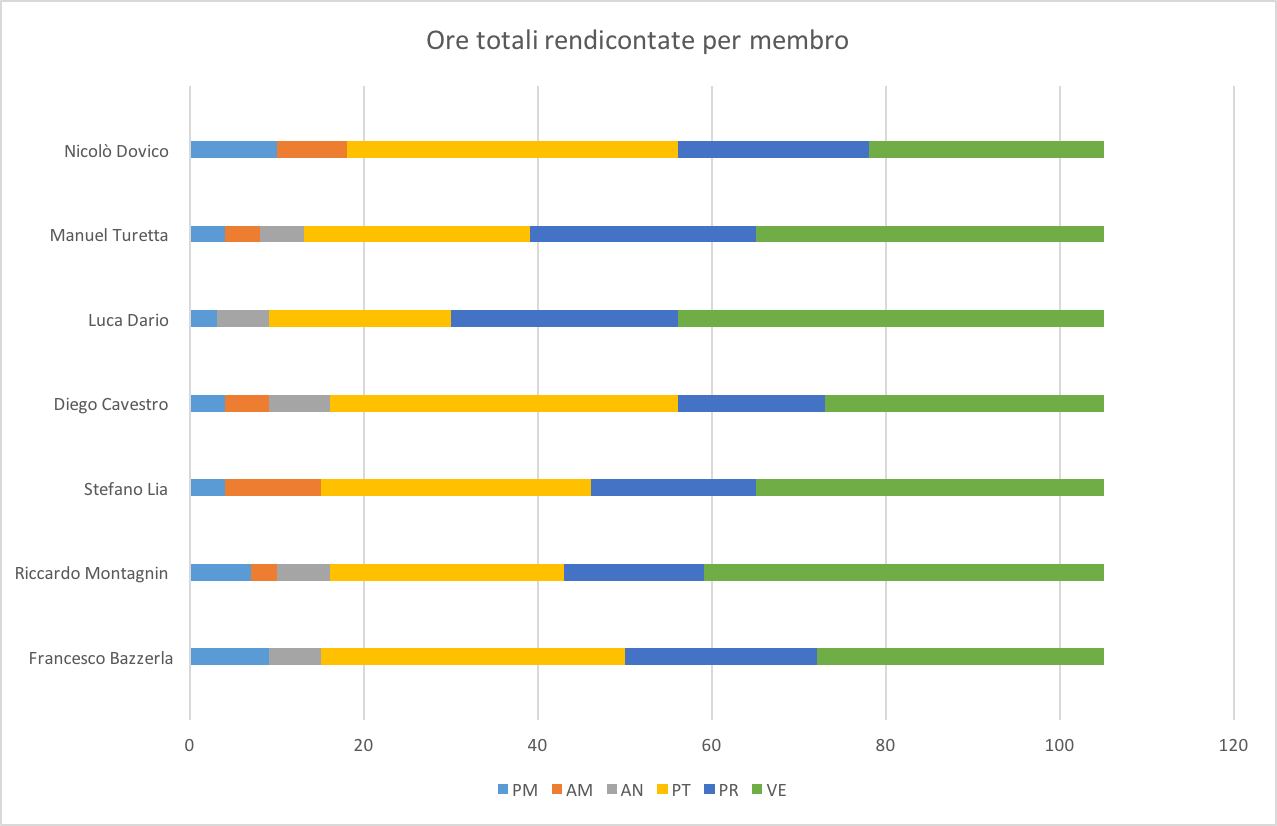
\includegraphics[scale=0.7]{Immagini/GraficiPianoLavoro/TOT.png}
	\caption{Incidenza ore totali per membro}
\end{figure}